\documentclass[../../main.tex]{subfiles}

\graphicspath{{../../image/}{../../figure/}}

\begin{document}

\section{通用图网络}\label{section:ch13-通用图网络}

迄今为止我们所考虑的图网络有许多变体和扩展。这里我们概述一些关键概念以及一些实践考虑。

\subsection{图注意力网络}\label{subsection:ch13-图注意力网络}

注意力机制在作为 Transformer 架构的基础时展现出强大的能力（参见\cref{section:ch12-注意力}）。在图神经网络中，注意力机制可以用于构建一种能够整合来自邻居节点信息的聚合函数。

\begin{definition}[图注意力网络]\label{definition:ch13-图注意力网络}
设 $\mathcal{G}=(\mathcal{V},\mathcal{E})$ 为简单无向图，$N=|\mathcal{V}|$，$\mathcal{N}(n)=\{m\in\mathcal{V}:\{n,m\}\in\mathcal{E}\}$ 非空；设第 $l$ 层的节点嵌入为 $\bm{h}_m^{(l)}\in\mathbb{R}^{D_l}$，嵌入维数 $D_l\geqslant1$，并对每一对满足 $m\in\mathcal{N}(n)$ 的节点给定实数 $A_{nm}\in\mathbb{R}$。若聚合量由
\begin{align}
\bm{z}_n^{(l)}=\operatorname{Aggregate}\!\left(\{\bm{h}_m^{(l)}:m\in\mathcal{N}(n)\}\right)=\sum_{m\in\mathcal{N}(n)}A_{nm}\,\bm{h}_m^{(l)}
\label{align:ch13-注意力聚合}
\end{align}
给出，且这些系数满足
\begin{align}
A_{nm}&\geqslant 0
\label{align:ch13-注意力非负}\\
\sum_{m\in\mathcal{N}(n)}A_{nm}&=1,
\label{align:ch13-注意力归一}
\end{align}
则把 $A_{nm}$ 称为节点 $n$ 分配给邻居节点 $m$ 的注意力系数，把按\eqref{align:ch13-注意力聚合}逐节点计算 $\bm{z}_n^{(l)}$ 的映射称为图注意力网络的聚合算子。条件\eqref{align:ch13-注意力非负}与\eqref{align:ch13-注意力归一}表明 $\bm{z}_n^{(l)}$ 是 $\{\bm{h}_m^{(l)}:m\in\mathcal{N}(n)\}$ 的凸组合，从而 $\|\bm{z}_n^{(l)}\|\leqslant\max_{m\in\mathcal{N}(n)}\|\bm{h}_m^{(l)}\|$；若某个节点满足 $\mathcal{N}(n)=\varnothing$，则\eqref{align:ch13-注意力归一}无定义，此时该节点的聚合量需另行规定。
\end{definition}

% SUPPLEMENT: parent=definition:ch13-图注意力网络; kind=motivation; location=紧随其后的 remark
\begin{remark}
\eqref{align:ch13-注意力非负}与\eqref{align:ch13-注意力归一}两条约束的作用不同：非负性使\eqref{align:ch13-注意力聚合}成为邻居嵌入的一个凸组合，因而聚合结果不会超出邻居嵌入的凸包，数值上不会因为正负抵消而失控；归一化使聚合量的尺度与邻居个数无关，避免了\eqref{align:ch13-求和聚合}中“度数越大、量级越大”的问题。两条合起来，$A_{nm}$ 可以被读作“节点 $n$ 把多少注意力分给邻居 $m$”的分配比例。\par
与\eqref{align:ch13-平均聚合}的固定权重 $1/|\mathcal{N}(n)|$ 相比，注意力权重是数据相关的：它由当前的嵌入计算得到，因此同一张图上不同样本、不同层的权重都可以不同。这正是原书所说的归纳偏置——某些相邻节点比其他节点更重要，而重要性由数据决定。\par
代价是计算量与存储量：每一条边都要算一个注意力系数，稠密图上这是 $O(N^2)$ 的量。此外，\eqref{align:ch13-注意力归一}的分母只对邻居求和，因此孤立节点的分母为 $0$，实际实现中需要补自环或特殊处理。
\end{remark}

这种网络称为图注意力网络（graph attention network）（Veličković et al., 2017），它可以捕获一种归纳偏置，该归纳偏置表明在确定最佳更新的过程中，某些相邻节点比其他节点更重要，而这种重要性取决于数据本身。

构建注意力系数的方法有很多种，但通常都会使用 softmax 函数。

\begin{definition}[注意力系数]\label{definition:ch13-注意力系数}
设 $\mathcal{G}=(\mathcal{V},\mathcal{E})$ 为简单无向图，$N=|\mathcal{V}|$，$\mathcal{N}(n)\neq\varnothing$ 对一切 $n\in\mathcal{V}$ 成立；设第 $l$ 层的节点嵌入为 $\bm{h}_m^{(l)}\in\mathbb{R}^{D}$，嵌入维数 $D\geqslant1$。若注意力系数按双线性得分取为
\begin{align}
A_{nm}=\frac{\exp\!\left(\bm{h}_n^{\mathsf T}\bm{W}\bm{h}_m\right)}{\sum_{m'\in\mathcal{N}(n)}\exp\!\left(\bm{h}_n^{\mathsf T}\bm{W}\bm{h}_{m'}\right)},
\label{align:ch13-双线性注意力}
\end{align}
其中 $\bm{W}\in\mathbb{R}^{D\times D}$ 为可学习参数矩阵，则把\eqref{align:ch13-双线性注意力}定义的 $A_{nm}$ 称为双线性注意力系数；此时 $A_{nm}>0$ 且 $\sum_{m\in\mathcal{N}(n)}A_{nm}=1$，故\eqref{align:ch13-注意力非负}与\eqref{align:ch13-注意力归一}自动成立。

更一般的构造是用一个神经网络组合边的两个端点的嵌入。设 $\operatorname{MLP}:\mathbb{R}^{D}\times\mathbb{R}^{D}\to\mathbb{R}$ 为可学习的标量函数，它在交换两个自变量时取值不变，即 $\operatorname{MLP}(\bm{u},\bm{v})=\operatorname{MLP}(\bm{v},\bm{u})$ 对一切 $\bm{u},\bm{v}\in\mathbb{R}^{D}$ 成立，且其参数在全部节点间共享。若
\begin{align}
A_{nm}=\frac{\exp\!\left\{\operatorname{MLP}(\bm{h}_n,\bm{h}_m)\right\}}{\sum_{m'\in\mathcal{N}(n)}\exp\!\left\{\operatorname{MLP}(\bm{h}_n,\bm{h}_{m'})\right\}},
\label{align:ch13-MLP注意力}
\end{align}
则把 $A_{nm}$ 称为由 $\operatorname{MLP}$ 诱导的注意力系数；同样有 $A_{nm}>0$ 与 $\sum_{m\in\mathcal{N}(n)}A_{nm}=1$。在上述共享参数与对称性条件下，以该系数代入\eqref{align:ch13-注意力聚合}所得的聚合算子在节点编号的置换下是等变的（见\cref{exercise:ch13-08}）。
\end{definition}

% SUPPLEMENT: parent=definition:ch13-注意力系数; kind=motivation; location=紧随其后的 remark
\begin{remark}
\eqref{align:ch13-双线性注意力}与\eqref{align:ch13-MLP注意力}都是“先算得分、再在邻域上做 softmax”的两步结构，区别只在得分函数。双线性形式的得分是 $\bm{h}_n^{\mathsf T}\bm{W}\bm{h}_m$，它对 $\bm{W}$ 线性，因而训练稳定、参数量只有 $D^2$；MLP 形式的得分是任意可学的标量函数，表达力更强但需要更多数据。\par
两条公式都自动满足\eqref{align:ch13-注意力非负}（指数函数为正）与\eqref{align:ch13-注意力归一}（softmax 分母的定义），因此定义中那两条约束不是额外假设，而是构造方式的直接结果。\par
定义中对 MLP 提出了一个不显眼但关键的要求：交换两个输入向量时输出不变。若 MLP 不对称，则 $A_{nm}\neq A_{mn}$，聚合将依赖“谁是被更新的节点”，这在无向图上没有意义，也会破坏等变性。双线性形式 $\bm{h}_n^{\mathsf T}\bm{W}\bm{h}_m$ 只有在 $\bm{W}$ 对称时才满足这一要求；原书未强调这一点，实现时若 $\bm{W}$ 取一般矩阵，得到的是有向注意力。
\end{remark}

\begin{proposition}[图注意力聚合的置换等变性]\label{proposition:ch13-图注意力等变性}
设注意力系数由\eqref{align:ch13-MLP注意力}给出，其中 MLP 在所有节点间共享且对两个输入向量对称，$\bm{P}$ 为任意置换矩阵。则按\eqref{align:ch13-注意力聚合}定义的聚合算子满足
\begin{align*}
\operatorname{Aggregate}\left(\{\bm{P}\bm{h}_m:m\in\mathcal{N}(n)\}\right)=\bm{P}\operatorname{Aggregate}\left(\{\bm{h}_m:m\in\mathcal{N}(n)\}\right),
\end{align*}
即该聚合函数在节点重新排序下是等变的。
\end{proposition}

\begin{proof}
记 $\widetilde{\bm{h}}_m=\bm{h}_{\pi^{-1}(m)}$，则按\eqref{align:ch13-MLP注意力}，重排后的注意力系数为
\begin{align*}
\widetilde{A}_{nm}&=\frac{\exp\{\operatorname{MLP}(\widetilde{\bm{h}}_n,\widetilde{\bm{h}}_m)\}}{\sum_{m'\in\widetilde{\mathcal{N}}(n)}\exp\{\operatorname{MLP}(\widetilde{\bm{h}}_n,\widetilde{\bm{h}}_{m'})\}}\\
&=\frac{\exp\{\operatorname{MLP}(\bm{h}_{\pi^{-1}(n)},\bm{h}_{\pi^{-1}(m)})\}}{\sum_{m'\in\widetilde{\mathcal{N}}(n)}\exp\{\operatorname{MLP}(\bm{h}_{\pi^{-1}(n)},\bm{h}_{\pi^{-1}(m')})\}},
\end{align*}
把分母中的求和变量换成 $m''=\pi^{-1}(m')$，则 $m''$ 遍历 $\mathcal{N}(\pi^{-1}(n))$，分母恰为 $\sum_{m''\in\mathcal{N}(\pi^{-1}(n))}\exp\{\operatorname{MLP}(\bm{h}_{\pi^{-1}(n)},\bm{h}_{m''})\}$，故 $\widetilde{A}_{nm}=A_{\pi^{-1}(n)\pi^{-1}(m)}$。这里用到 MLP 在所有节点间共享（分子分母中的 MLP 是同一个函数）这一事实。于是
\begin{align*}
\widetilde{\bm{z}}_n&=\sum_{m\in\widetilde{\mathcal{N}}(n)}\widetilde{A}_{nm}\widetilde{\bm{h}}_m=\sum_{m\in\widetilde{\mathcal{N}}(n)}A_{\pi^{-1}(n)\pi^{-1}(m)}\bm{h}_{\pi^{-1}(m)}\\
&=\sum_{m''\in\mathcal{N}(\pi^{-1}(n))}A_{\pi^{-1}(n)m''}\bm{h}_{m''}=\bm{z}_{\pi^{-1}(n)},
\end{align*}
第二个等号是重指标 $m''=\pi^{-1}(m)$。这恰是 $\widetilde{\bm{z}}=\bm{P}\bm{z}$，即聚合算子与置换矩阵可交换。证毕。
\end{proof}

% SUPPLEMENT: parent=proposition:ch13-图注意力等变性; kind=motivation; location=紧随其后的 remark
\begin{remark}
证明中真正用到对称性的地方只有一处：把 $\widetilde{A}_{nm}$ 的分子写成 $\operatorname{MLP}(\bm{h}_{\pi^{-1}(n)},\bm{h}_{\pi^{-1}(m)})$ 时，两个参数的位置必须与原式一致。若 MLP 不对称，重排会让“查询向量”与“键向量”的角色互换，$A_{nm}$ 与 $A_{mn}$ 不再相等，聚合结果依赖于节点编号的方向，等变性随之失效。\par
命题没有断言 $\bm{z}_n$ 对邻居的置换不变——它不是不变的，而是等变的：重排节点后，第 $n$ 个分量变成原来的第 $\pi^{-1}(n)$ 个分量。这正是\eqref{align:ch13-置换等变性}要求的行为。\par
把本命题与\cref{theorem:ch13-图网络等变性}结合可知，用注意力聚合替换求和聚合不会破坏整个网络的等变性，因此图注意力网络可以任意堆叠。原书把这一验证留作\cref{exercise:ch13-08}，这里给出完整论证以便后续引用。
\end{remark}

\begin{definition}[多头图注意力]\label{definition:ch13-多头图注意力}
设 $\mathcal{G}=(\mathcal{V},\mathcal{E})$ 为简单无向图，$N=|\mathcal{V}|$，$\mathcal{N}(n)\neq\varnothing$；设第 $l$ 层的节点嵌入为 $\bm{h}_m^{(l)}\in\mathbb{R}^{D}$，嵌入维数 $D\geqslant1$；设头数 $H\geqslant1$，每个头的输出维数 $D_h\geqslant1$。对每个头 $h=1,\cdots,H$，设 $A_{nm}^{(h)}$ 为按\eqref{align:ch13-双线性注意力}或\eqref{align:ch13-MLP注意力}独立计算、并满足\eqref{align:ch13-注意力非负}与\eqref{align:ch13-注意力归一}的注意力系数，各头使用互不相同的参数集；设 $\bm{W}^{(h)}\in\mathbb{R}^{D_h\times D}$ 为该头的权重矩阵，$\bm{W}_{\mathrm{out}}\in\mathbb{R}^{D_{\mathrm{out}}\times(HD_h)}$ 为可学习的投影矩阵，$D_{\mathrm{out}}\geqslant1$。若该层的输出由先逐头聚合、再拼接、最后投影给出，即
\begin{align*}
\bm{z}_n^{(l)}=\bm{W}_{\mathrm{out}}\begin{pmatrix}\bm{z}_n^{(1)}\\ \vdots\\ \bm{z}_n^{(H)}\end{pmatrix},\qquad \bm{z}_n^{(h)}=\sum_{m\in\mathcal{N}(n)}A_{nm}^{(h)}\bm{W}^{(h)}\bm{h}_m^{(l)},
\end{align*}
则把该聚合层称为 $H$ 头图注意力层（参见\cref{subsection:ch12-多头注意力}），把每个 $h$ 称为一个注意力头。若图是完全图，即 $\mathcal{N}(n)=\mathcal{V}\setminus\{n\}$ 对一切 $n$ 成立，则该层化为标准的 Transformer 自注意力编码层（见\cref{exercise:ch13-09}）。
\end{definition}

% SUPPLEMENT: parent=definition:ch13-多头图注意力; kind=motivation; location=紧随其后的 remark
\begin{remark}
多头的意义在于让不同的头关注邻域中不同的关系模式：一个头可能按化学键类型分配注意力，另一个头可能按原子距离分配，最后的拼接与线性投影把这些视角合并。这与卷积网络中一层使用多个滤波器完全平行。\par
每个头必须有自己独立的参数集，否则 $H$ 个头会退化为同一个头，只是把结果重复了 $H$ 次。拼接使输出维数变为 $H$ 倍（当每个头输出 $D/H$ 维时恰好回到 $D$ 维），线性投影则负责把拼接结果映射回所需的维数并混合各头的信息。\par
“全连接图上多头图注意力即 Transformer 编码器”这一断言的确切含义与证明见\cref{exercise:ch13-09}：在完全图上邻居集合就是除自身外的全部节点，softmax 注意力与 Transformer 的自注意力在形式上一致，差别只在是否包含自身以及缩放因子的写法。
\end{remark}

\subsection{边嵌入}\label{subsection:ch13-边嵌入}

前面讨论的图神经网络使用的嵌入向量都与节点相关联。我们已经看到一些网络也具有与边相关联的数据。即使不存在与边相关联的观测值，我们也仍然可以维护和更新基于边的隐藏变量，这些变量可以为图神经网络学习的内部表示做出贡献。除了由 $\bm{h}_n^{(l)}$ 给出的节点嵌入，我们还引入了边嵌入 $\bm{e}_{nm}^{(l)}$。

\begin{definition}[带边嵌入的消息传递]\label{definition:ch13-边嵌入消息传递}
设 $\mathcal{G}=(\mathcal{V},\mathcal{E})$ 为简单无向图，$N=|\mathcal{V}|$，$L\geqslant1$ 为层数；设第 $l$ 层的节点嵌入为 $\bm{h}_n^{(l)}\in\mathbb{R}^{D_l}$、边嵌入为 $\bm{e}_{nm}^{(l)}\in\mathbb{R}^{E_l}$，其中 $\bm{e}_{nm}^{(l)}$ 对每条边 $\{n,m\}\in\mathcal{E}$ 给出并满足 $\bm{e}_{nm}^{(l)}=\bm{e}_{mn}^{(l)}$，维数 $D_l\geqslant1$、$E_l\geqslant1$。给定三个映射 $\operatorname{Update}_{\mathrm{edge}}:\mathbb{R}^{E_l}\times\mathbb{R}^{D_l}\times\mathbb{R}^{D_l}\to\mathbb{R}^{E_{l+1}}$、$\operatorname{Aggregate}_{\mathrm{node}}:\mathcal{M}(\mathbb{R}^{E_{l+1}})\to\mathbb{R}^{E_{l+1}}$、$\operatorname{Update}_{\mathrm{node}}:\mathbb{R}^{D_l}\times\mathbb{R}^{E_{l+1}}\to\mathbb{R}^{D_{l+1}}$，其中 $\mathcal{M}(\mathbb{R}^{d})$ 表示由 $\mathbb{R}^{d}$ 中向量的有限多重集构成的集合，且三个映射的参数在全部节点与边上共享。若对 $l=0,\cdots,L-1$ 依次计算
\begin{align}
\bm{e}_{nm}^{(l+1)}&=\operatorname{Update}_{\mathrm{edge}}\!\left(\bm{e}_{nm}^{(l)},\bm{h}_n^{(l)},\bm{h}_m^{(l)}\right),
\label{align:ch13-边更新}\\
\bm{z}_n^{(l+1)}&=\operatorname{Aggregate}_{\mathrm{node}}\!\left(\{\bm{e}_{nm}^{(l+1)}:m\in\mathcal{N}(n)\}\right),
\label{align:ch13-边聚合}\\
\bm{h}_n^{(l+1)}&=\operatorname{Update}_{\mathrm{node}}\!\left(\bm{h}_n^{(l)},\bm{z}_n^{(l+1)}\right),
\label{align:ch13-边节点更新}
\end{align}
则把由这三式复合而成的一层称为带边嵌入的消息传递层，并称 $\bm{e}_{nm}^{(L)}$ 为最终层的边嵌入，它可直接用于预测与边相关的量。三式的执行次序固定为“先更新边、再由边聚合、最后更新节点”，\eqref{align:ch13-边聚合}中的求和项取本层更新后的 $\bm{e}_{nm}^{(l+1)}$。
\end{definition}

% SUPPLEMENT: parent=definition:ch13-边嵌入消息传递; kind=motivation; location=紧随其后的 remark
\begin{remark}
这三式相对\eqref{align:ch13-聚合定义}与\eqref{align:ch13-更新定义}的推广在于多了一层“边”：消息不再直接取邻居的节点嵌入，而是先由两端节点的嵌入生成一个边向量，再从边向量聚合到节点。这样做的收益是表示能力的提升——边向量可以编码“这两个节点之间的关系类型”，而仅用节点嵌入的求和无法区分“同一条消息来自不同类型的边”。\par
三式的执行顺序不能随意交换：\eqref{align:ch13-边聚合}用的是 $\bm{e}_{nm}^{(l+1)}$ 而不是 $\bm{e}_{nm}^{(l)}$，即先更新边、再聚合边、最后更新节点。若改成先聚合旧边再更新边，则本层的节点更新用不到本层的边信息，表达力下降。\par
$\bm{e}_{nm}$ 的下标是有序对 $(n,m)$，但无向图中 $(n,m)$ 与 $(m,n)$ 是同一条边，因此实现时必须保证 $\bm{e}_{nm}=\bm{e}_{mn}$，否则等变性会被破坏。原书写成 $\bm{e}_{nm}$ 是记号上的简化。
\end{remark}

\subsection{图嵌入}\label{subsection:ch13-图嵌入}

除了节点嵌入和边嵌入，我们还可以维护和更新与整个图相关的嵌入向量 $\bm{g}^{(l)}$。将所有这些方面结合在一起，我们便能够为图结构化应用定义更通用的一组消息传递函数，以及更丰富的学习表示集合。

\begin{definition}[通用图网络的消息传递方程]\label{definition:ch13-通用消息传递}
设 $\mathcal{G}=(\mathcal{V},\mathcal{E})$ 为简单无向图，$N=|\mathcal{V}|$，$L\geqslant1$ 为层数；设第 $l$ 层的节点嵌入为 $\bm{h}_n^{(l)}\in\mathbb{R}^{D_l}$、边嵌入为 $\bm{e}_{nm}^{(l)}\in\mathbb{R}^{E_l}$（对每条 $\{n,m\}\in\mathcal{E}$ 给出，且 $\bm{e}_{nm}^{(l)}=\bm{e}_{mn}^{(l)}$）、图嵌入为 $\bm{g}^{(l)}\in\mathbb{R}^{G_l}$，各维数 $D_l,E_l,G_l\geqslant1$。给定四个映射
\begin{align*}
&\operatorname{Update}_{\mathrm{edge}}:\mathbb{R}^{E_l}\times\mathbb{R}^{D_l}\times\mathbb{R}^{D_l}\times\mathbb{R}^{G_l}\to\mathbb{R}^{E_{l+1}},\\
&\operatorname{Aggregate}_{\mathrm{node}}:\mathcal{M}(\mathbb{R}^{E_{l+1}})\to\mathbb{R}^{E_{l+1}},\\
&\operatorname{Update}_{\mathrm{node}}:\mathbb{R}^{D_l}\times\mathbb{R}^{E_{l+1}}\times\mathbb{R}^{G_l}\to\mathbb{R}^{D_{l+1}},\\
&\operatorname{Update}_{\mathrm{graph}}:\mathbb{R}^{G_l}\times\mathcal{M}(\mathbb{R}^{D_{l+1}})\times\mathcal{M}(\mathbb{R}^{E_{l+1}})\to\mathbb{R}^{G_{l+1}},
\end{align*}
其中 $\mathcal{M}(\mathbb{R}^{d})$ 表示由 $\mathbb{R}^{d}$ 中向量的有限多重集构成的集合，四个映射的参数在全部节点与边上共享。若对 $l=0,\cdots,L-1$ 依次计算
\begin{align}
\bm{e}_{nm}^{(l+1)}&=\operatorname{Update}_{\mathrm{edge}}\!\left(\bm{e}_{nm}^{(l)},\bm{h}_n^{(l)},\bm{h}_m^{(l)},\bm{g}^{(l)}\right),
\label{align:ch13-通用边更新}\\
\bm{z}_n^{(l+1)}&=\operatorname{Aggregate}_{\mathrm{node}}\!\left(\{\bm{e}_{nm}^{(l+1)}:m\in\mathcal{N}(n)\}\right),
\label{align:ch13-通用边聚合}\\
\bm{h}_n^{(l+1)}&=\operatorname{Update}_{\mathrm{node}}\!\left(\bm{h}_n^{(l)},\bm{z}_n^{(l+1)},\bm{g}^{(l)}\right),
\label{align:ch13-通用节点更新}\\
\bm{g}^{(l+1)}&=\operatorname{Update}_{\mathrm{graph}}\!\left(\bm{g}^{(l)},\{\bm{h}_n^{(l+1)}:n\in\mathcal{V}\},\{\bm{e}_{nm}^{(l+1)}:(n,m)\in\mathcal{E}\}\right),
\label{align:ch13-通用图更新}
\end{align}
则把由这四式复合而成的一层称为通用图网络的消息传递层（Battaglia et al., 2018）。四式按边、节点、图的次序依次更新，且 $\operatorname{Update}_{\mathrm{graph}}$ 的两个集合自变量以多重集的形式传入，故它对节点与边的枚举次序不变。
\end{definition}

% SUPPLEMENT: parent=definition:ch13-通用消息传递; kind=motivation; location=紧随其后的 remark
\begin{remark}
这四式把“节点—边—图”三个层次的变量放进同一个更新回路，是本章最一般的消息传递形式；前面所有的模型都是它的特例：去掉 $\bm{g}$ 与边变量就回到\eqref{align:ch13-聚合定义}，保留边变量但去掉 $\bm{g}$ 就回到\eqref{align:ch13-边更新}。理解这一点比记住四式更重要——它说明这些模型之间的差别只是“哪些变量参与更新”，而不是彼此无关的四种算法。\par
四个更新函数的输入各不相同，这决定了信息流的顺序：边只知道两端节点与全局状态，节点知道自身、邻域聚合与全局状态，全局变量则能看到全部节点与全部边。因此 $\bm{g}$ 是唯一“全局可见”的变量，它承担把远距离信息压缩传递的角色；这也是为什么原书在讨论过度平滑时提到的“超级节点”与 $\bm{g}$ 有相似的作用。\par
\eqref{align:ch13-通用图更新}的输入是集合 $\{\bm{h}_n^{(l+1)}\}$ 与 $\{\bm{e}_{nm}^{(l+1)}\}$，因此 $\operatorname{Update}_{\mathrm{graph}}$ 必须是置换不变的，否则整个网络的图级表示会依赖节点编号。这一点是\eqref{align:ch13-图级读出}中求和要求的同一件事，只是发生在每一层而不是只在最后一层。
\end{remark}

这些消息传递方程首先更新边嵌入向量 $\bm{e}_{nm}^{(l+1)}$，该操作是基于边嵌入向量的先前状态，每条边连接的节点的嵌入向量，以及图级嵌入向量 $\bm{g}^{(l)}$ 进行的，参见\eqref{align:ch13-通用边更新}。然后将这些更新的边嵌入向量在连接到每个节点的每条边上进行聚合，参见\eqref{align:ch13-通用边聚合}。接下来转而利用当前节点的嵌入向量和图级嵌入向量更新节点嵌入向量 $\bm{h}_n^{(l+1)}$，参见\eqref{align:ch13-通用节点更新}。最后基于图中所有节点和所有边的信息，以及从前一层获得的图级嵌入向量，更新当前层的图级嵌入向量。\cref{figure:ch13-消息传递更新}演示了上述过程，算法 13.2 对图消息传递更新做了总结。

\begin{figure}[htbp]
  \centering
  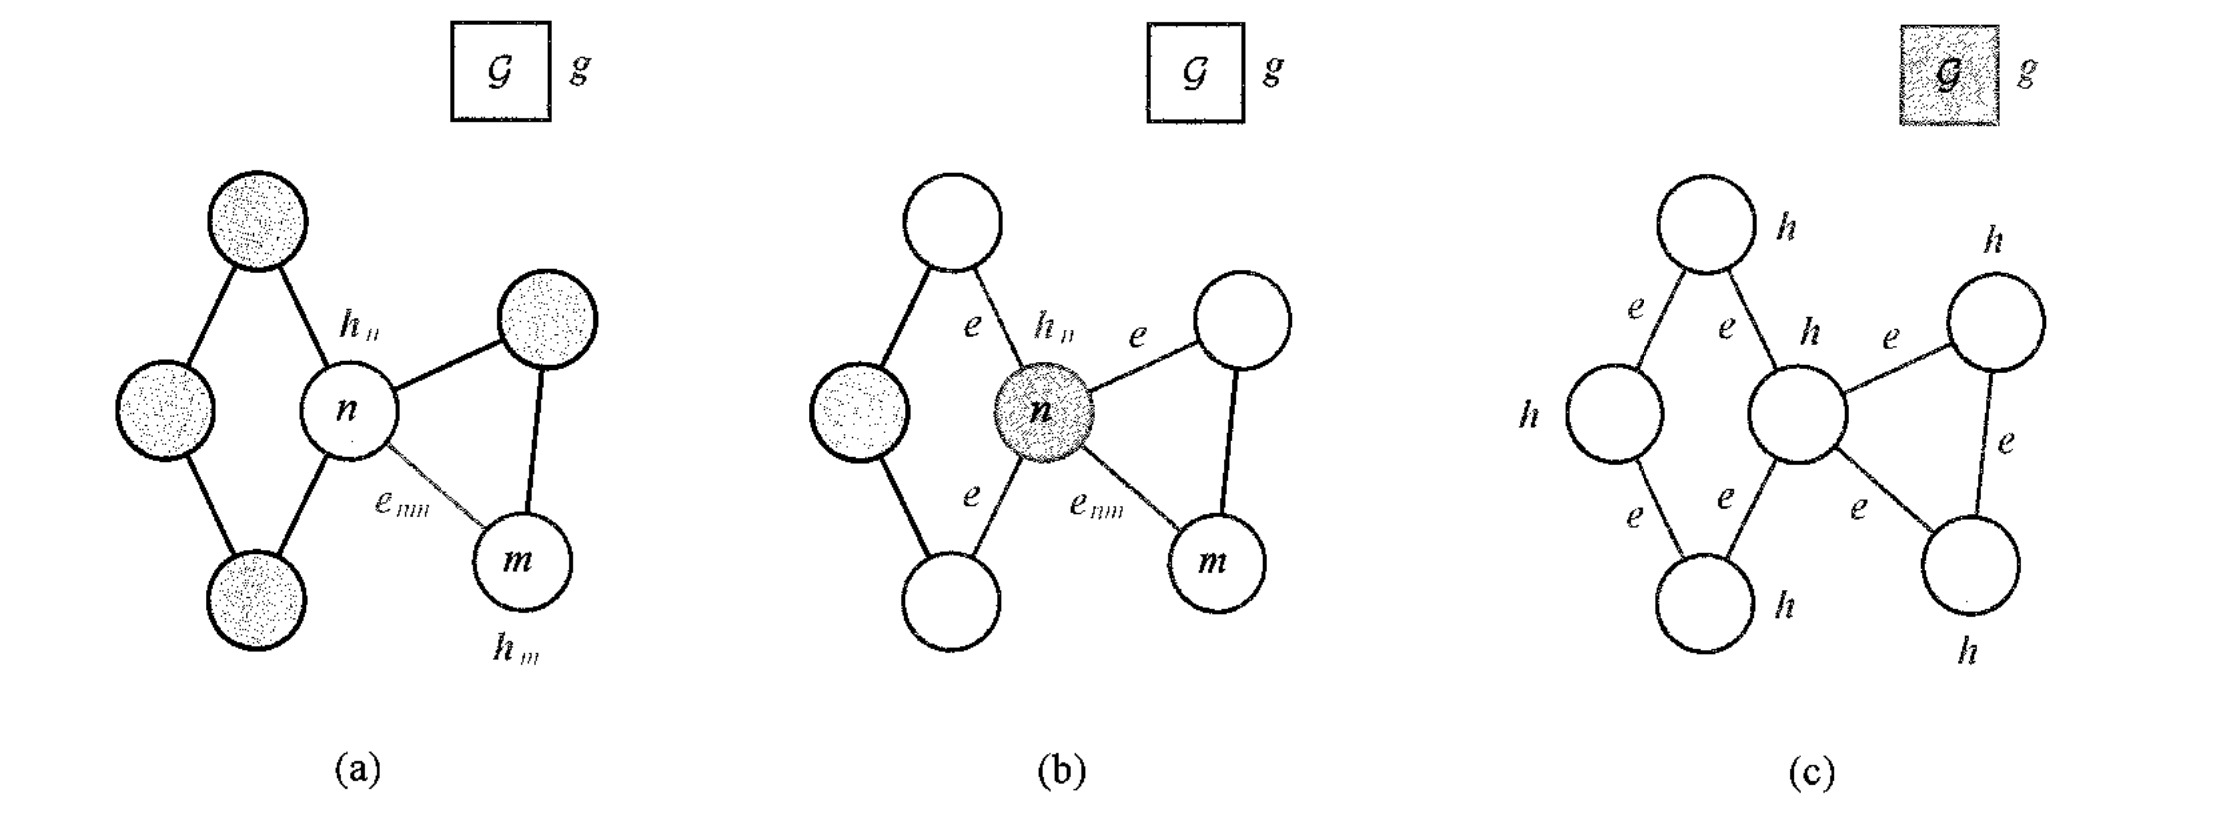
\includegraphics[width=0.95\textwidth]{ch13-fig13.5-msg-update.png}
  \caption{\eqref{align:ch13-通用边更新}～\eqref{align:ch13-通用图更新}定义的图消息传递更新的示意图，展示了 (a) 边更新、(b) 节点更新，以及 (c) 全局图更新。在每种情况下，正在更新的变量用红色显示，而那些对该更新有贡献的变量则用蓝色显示}
  \label{figure:ch13-消息传递更新}
\end{figure}

\begin{center}
\fbox{\begin{minipage}{0.9\textwidth}
\small
\textbf{算法 13.2：图消息传递更新}\par\smallskip
\textbf{输入：}无向图 $\mathcal{G}=(\mathcal{V},\mathcal{E})$；初始节点嵌入 $\{\bm{h}_n^{(0)}\}$；初始边嵌入 $\{\bm{e}_{nm}^{(0)}\}$；初始图嵌入 $\bm{g}^{(0)}$\par
\textbf{输出：}最终节点嵌入 $\{\bm{h}_n^{(L)}\}$；最终边嵌入 $\{\bm{e}_{nm}^{(L)}\}$；最终图嵌入 $\bm{g}^{(L)}$\par
\smallskip
\hrule\smallskip
\emph{// 迭代地进行消息传递}\\
\textbf{for} $l\in\{0,\cdots,L-1\}$ \textbf{do}\\
\hspace*{2em}$\bm{e}_{nm}^{(l+1)}\leftarrow\operatorname{Update}_{\mathrm{edge}}\left(\bm{e}_{nm}^{(l)},\bm{h}_n^{(l)},\bm{h}_m^{(l)},\bm{g}^{(l)}\right)$\\
\hspace*{2em}$\bm{z}_n^{(l+1)}\leftarrow\operatorname{Aggregate}_{\mathrm{node}}\left(\{\bm{e}_{nm}^{(l+1)}:m\in\mathcal{N}(n)\}\right)$\\
\hspace*{2em}$\bm{h}_n^{(l+1)}\leftarrow\operatorname{Update}_{\mathrm{node}}\left(\bm{h}_n^{(l)},\bm{z}_n^{(l+1)},\bm{g}^{(l)}\right)$\\
\hspace*{2em}$\bm{g}^{(l+1)}\leftarrow\operatorname{Update}_{\mathrm{graph}}\left(\bm{g}^{(l)},\{\bm{h}_n^{(l+1)}\},\{\bm{e}_{nm}^{(l+1)}\}\right)$\\
\textbf{end for}\\
\textbf{return} $\{\bm{h}_n^{(L)}\},\{\bm{e}_{nm}^{(L)}\},\bm{g}^{(L)}$
\end{minipage}}
\end{center}

\end{document}
